\documentclass[a4paper]{article}

\usepackage[utf8]{inputenc}
\usepackage[T1]{fontenc}
\usepackage{textcomp}
\usepackage{amsmath, amssymb}
\usepackage{float}


% figure support
\usepackage{import}
\usepackage{xifthen}
\pdfminorversion=7
\usepackage{pdfpages}
\usepackage{transparent}
\newcommand{\incfig}[1]{%
	\def\svgwidth{\columnwidth}
	\import{./figures/}{#1.pdf_Tex}
}

\pdfsuppresswarningpagegroup=1

\title{Introduction to Formal Linguistics - Homework 2}
\date{\today}
\author{Andrew McIsaac}

\begin{document}
\maketitle

\begin{enumerate}
\item %  1  %



Valency Frame 1 [to scan through]: ACT$^{obl}$, PAT$^{obl}$
	
Valency Frame 2 [to look around]: ACT$^{obl}$, PAT$^{opt}$, LOC$^{obl}$

Valency Frame 3 [to feed (generally for an animal)]: ACT$^{obl}$, PAT$^{opt}$

ACT, PAT are arguments, and LOC is an adjunct.

Valency Frame 1 is used in the sense of searching through a specific object
(e.g. a book), as in Sentence 1 "The browser will browse documentation notes."
It requires that something (the patient) be browsed, and that someone is doing
the browsing (the actor).

Valency Frame 2 is used in the sense of wandering around a place or among items,
looking at what is there but not looking for a specific item. In the case where
the patient is not specified, the obligatory location becomes the patient
because of argument shifting. For example, in Sentence 7 "The remainder of the
evening is yours to browse among the antiques", the location "among the 
antiques" becomes the patient. Compare this to Sentence 20, where the location
is the department stores, and the patient (the thing that is being browsed) is
the fabrics.

Valency Frame 3 is used for animals (mainly) that are grazing or feeding on
something. What is being grazed does not need to be specified, as in Sentence
11 "The elephant drivers are often encouraged by tourists or tour operators to 
move in very close to browsing rhinos".
\item %  2  %

\textit{to browse} equivalents in German: \textit{abfressen} (to graze) and
\textit{durchstöbern} (to scan through).

\textit{abfressen}: ACT$^{obl}$, PAT$^{obl}$

"Immer schön sind künstliche Terrarienpflanzen, die die Bartagamen auch nicht
anknabbern oder abfressen können." (Artificial terrarium plants that bearded
dragons cannot nibble on or browse are beautiful.)

%"Der Koala frisst auf dem Eukalyptus ab." (The koala browses on the eucalyptus.)

\textit{durchstöbern}: ACT$^{obl}$, PAT$^{obl}$, AIM$^{opt}$

%"Ich habe im Wörterbuch durchgestöbert." (I browsed through the dictionary.)

"Für live Angebote empfehle ich, Facebook und Instagram nach Aktivitäten,
die Ihr Kind mag, zu durchstöbern." (For active listings I recommend browsing 
Facebook and Instagram for activities that your child likes.)

\item %  3  %

`also' is defined as `RHEM' because of its function for indicating newly added
information after the word (i.e. `the browser will already do some things, and
it will \textbf{also} browse documentation notes').


	\begin{figure}[H]
		\centering
		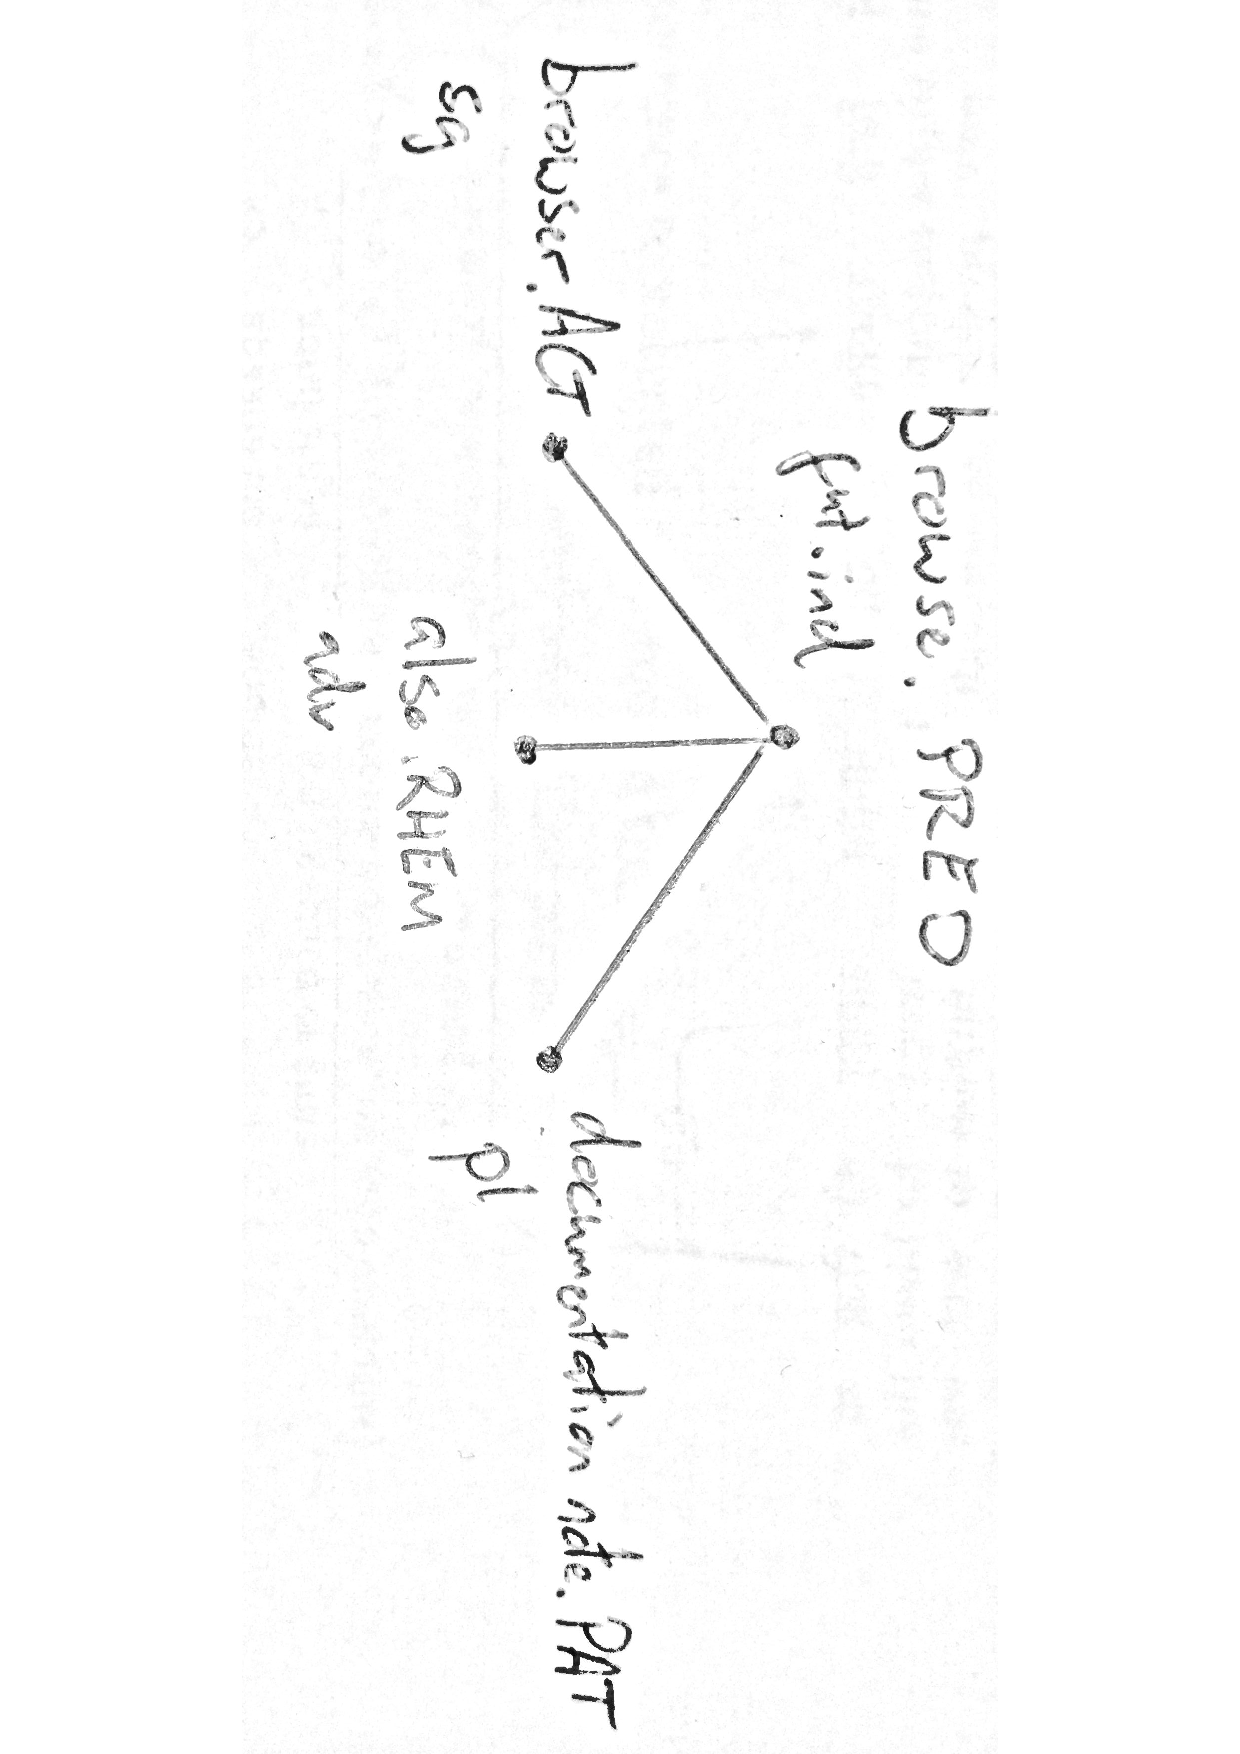
\includegraphics[width=0.7\textwidth, angle=90]{browse_fgd.pdf}
%		\caption{}
		\label{fig:fgd}
	\end{figure}

\item %  4  $

	"The browser also browsed documentation notes."

	"The browsers will also browse documentation notes."


\end{enumerate}


\end{document}
